\section{Objetivos}
Nesta prática objetiva-se apresentar os princípios elementares para amostragem de sinais
\section{Fundamentação Teórica}

Sendo o sinal analógico contínuo no tempo e amplitude, contém uma infinidade de valores. O aparelhos de processamento digital possuem uma banda passante limitada, acarretando na finitude de amostras utilizada para formação do sinal. 

A amostragem de um sinal analógico é caracterizada como o processo pelo qual o mesmo é representado por um conjunto discreto de números. Este número, ou amostras, são iguais ao valor no sinal neste respectivo instante. A quantidade de amostras é definida pela frequência de amostragem (frequência de coleta dos valores) comparado a frequência fundamental do sinal.

A escolha da frequência de amostragem é baseado no \textit{Teorema de amostragem de Nyquist e Shannon}. Este teorema basicamente estabelece que o sinal é precisamente  reconstruído por amostras sob a condição que componente de maior frequência não deve ser maior que metade da taxa de amostragem.

Quando este teorema não é obedecido, ocorre \textit{folding} e/ou \textit{aliasing}, fenômeno de sobreposição do espectro de frequência conhecido. Um filtro anti-\textit{aliasing }analógico é frequentemente colocado entre o sensor e o conversor A/D tendo como função, a redução das componentes de ruídos em alta frequência
\section{Procedimentos}
O exercício consistiu em utilizar o $Simulink^{\textregistered}$ para a construção do sinal contínuo no tempos com as seguintes  componentes frequências:

\begin{itemize}
	\item $f_0$ = 1 Hz;
	\item $f_1$ = 5 Hz;
	\item $f_2$ = 100 Hz; 
\end{itemize}

Sendo estes sinais amostrados  por um filtro \textit{Zero-order-hold} (ZOH) com as seguintes frequências de amostragem ($f_s$):

\begin{itemize}
	\item $f_{s1}$ = 10 Hz;
	\item $f_{s2}$ = 100 Hz;
	\item $f_{s3}$ = 1000 Hz; 
\end{itemize}

Na análise do espectro foi utilizado o comando FFT do $Matlab^{\textregistered}$, de forma a verificar o fenômeno de \textit{aliasing}	 para cada caso da frequência de amostragem. Para as frequências onde ocorreram  foi projeto um filtro passa-baixa.


\section{Resultados e discursões}

\begin{figure}[!th]
	\centering
	\includegraphics[scale = .55]{Imagens/pratica4_1.PNG}
	\caption{Diagrama de blocos da prática 4.}
	\label{fig:pr4_esquema}
\end{figure}

\begin{figure}[!th]
	\centering
	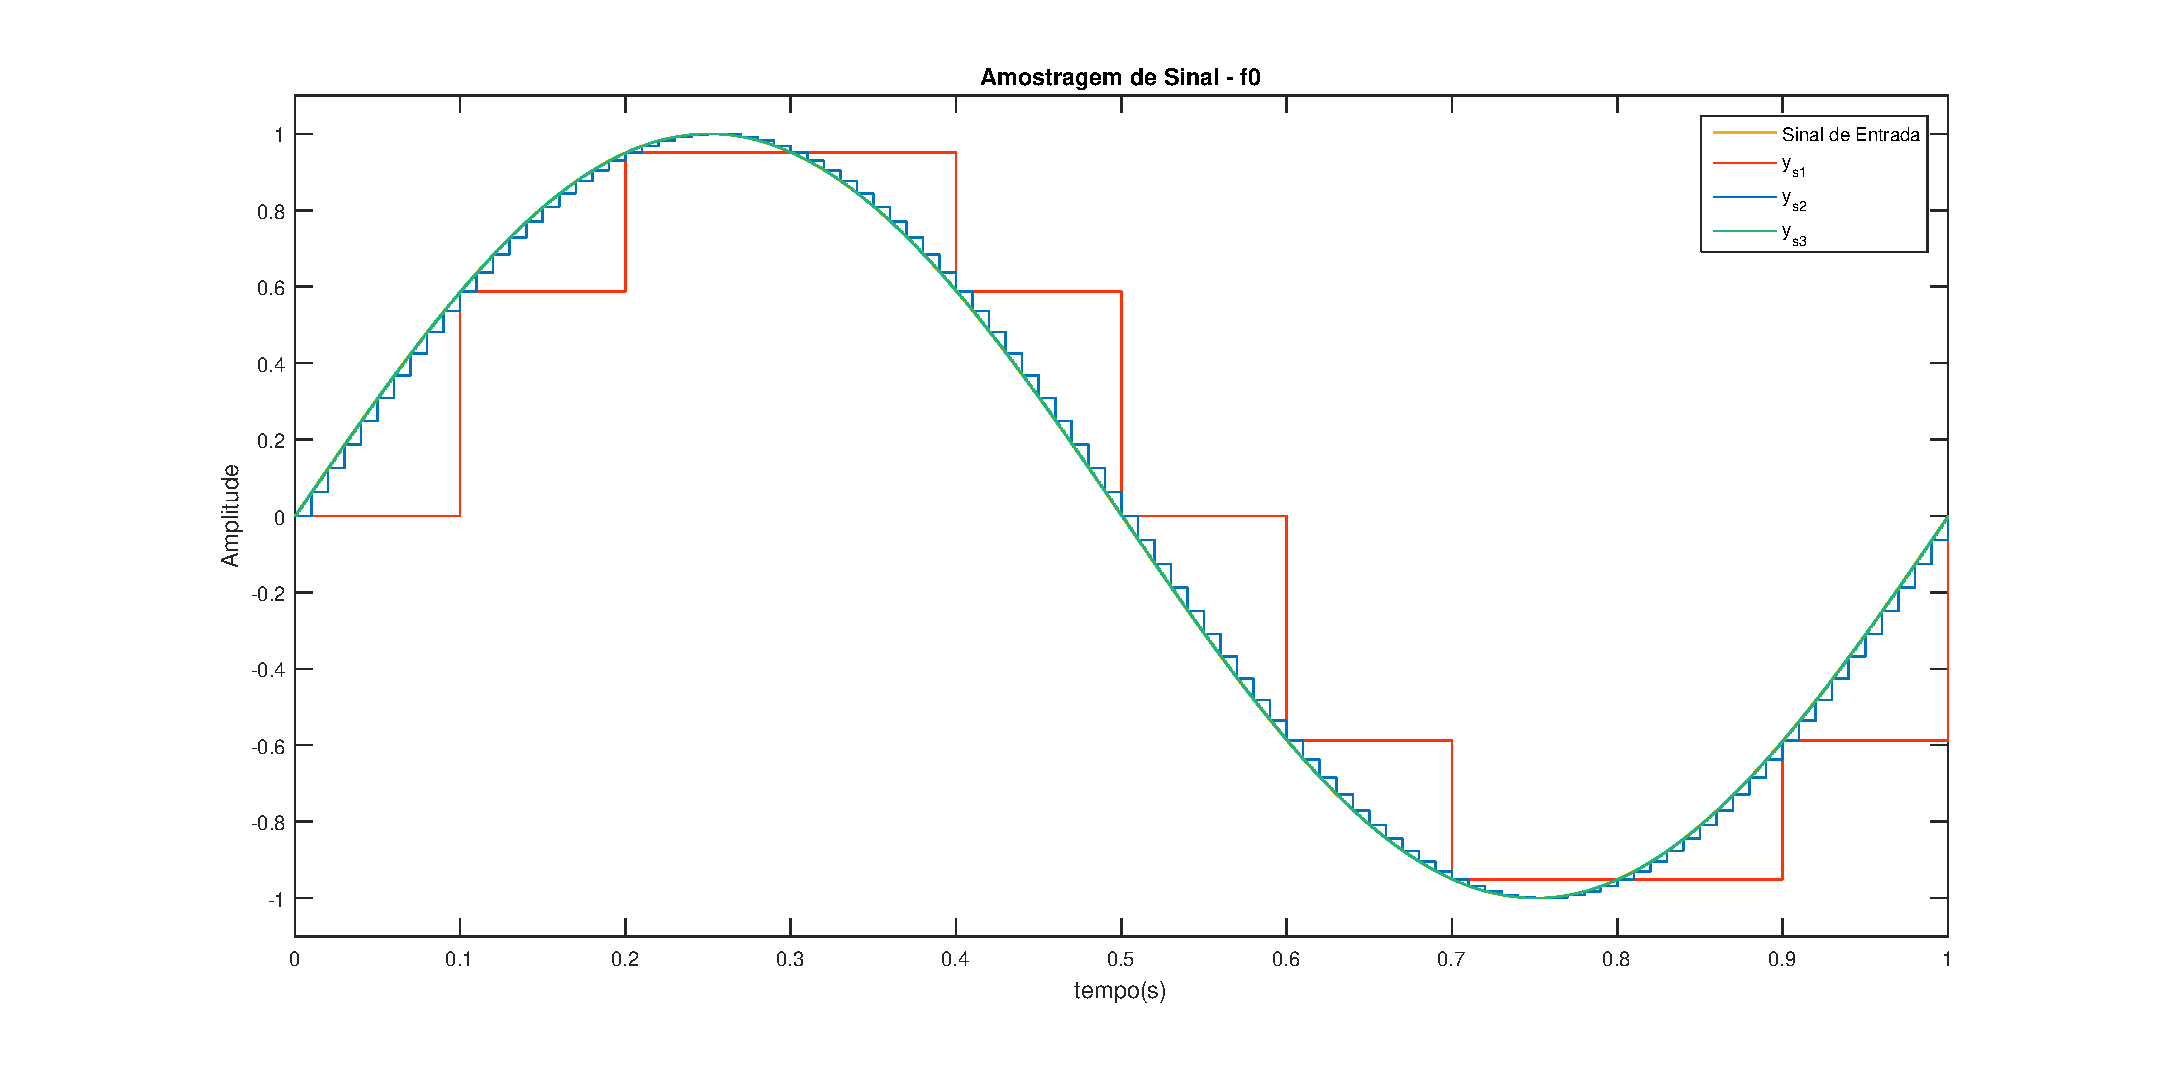
\includegraphics[scale = .45]{Imagens/pratica4_2.eps}
	\caption{Diagrama de blocos da prática 4.}
	\label{fig:pr4_esquema}
\end{figure}

\begin{figure}[!th]
	\centering
	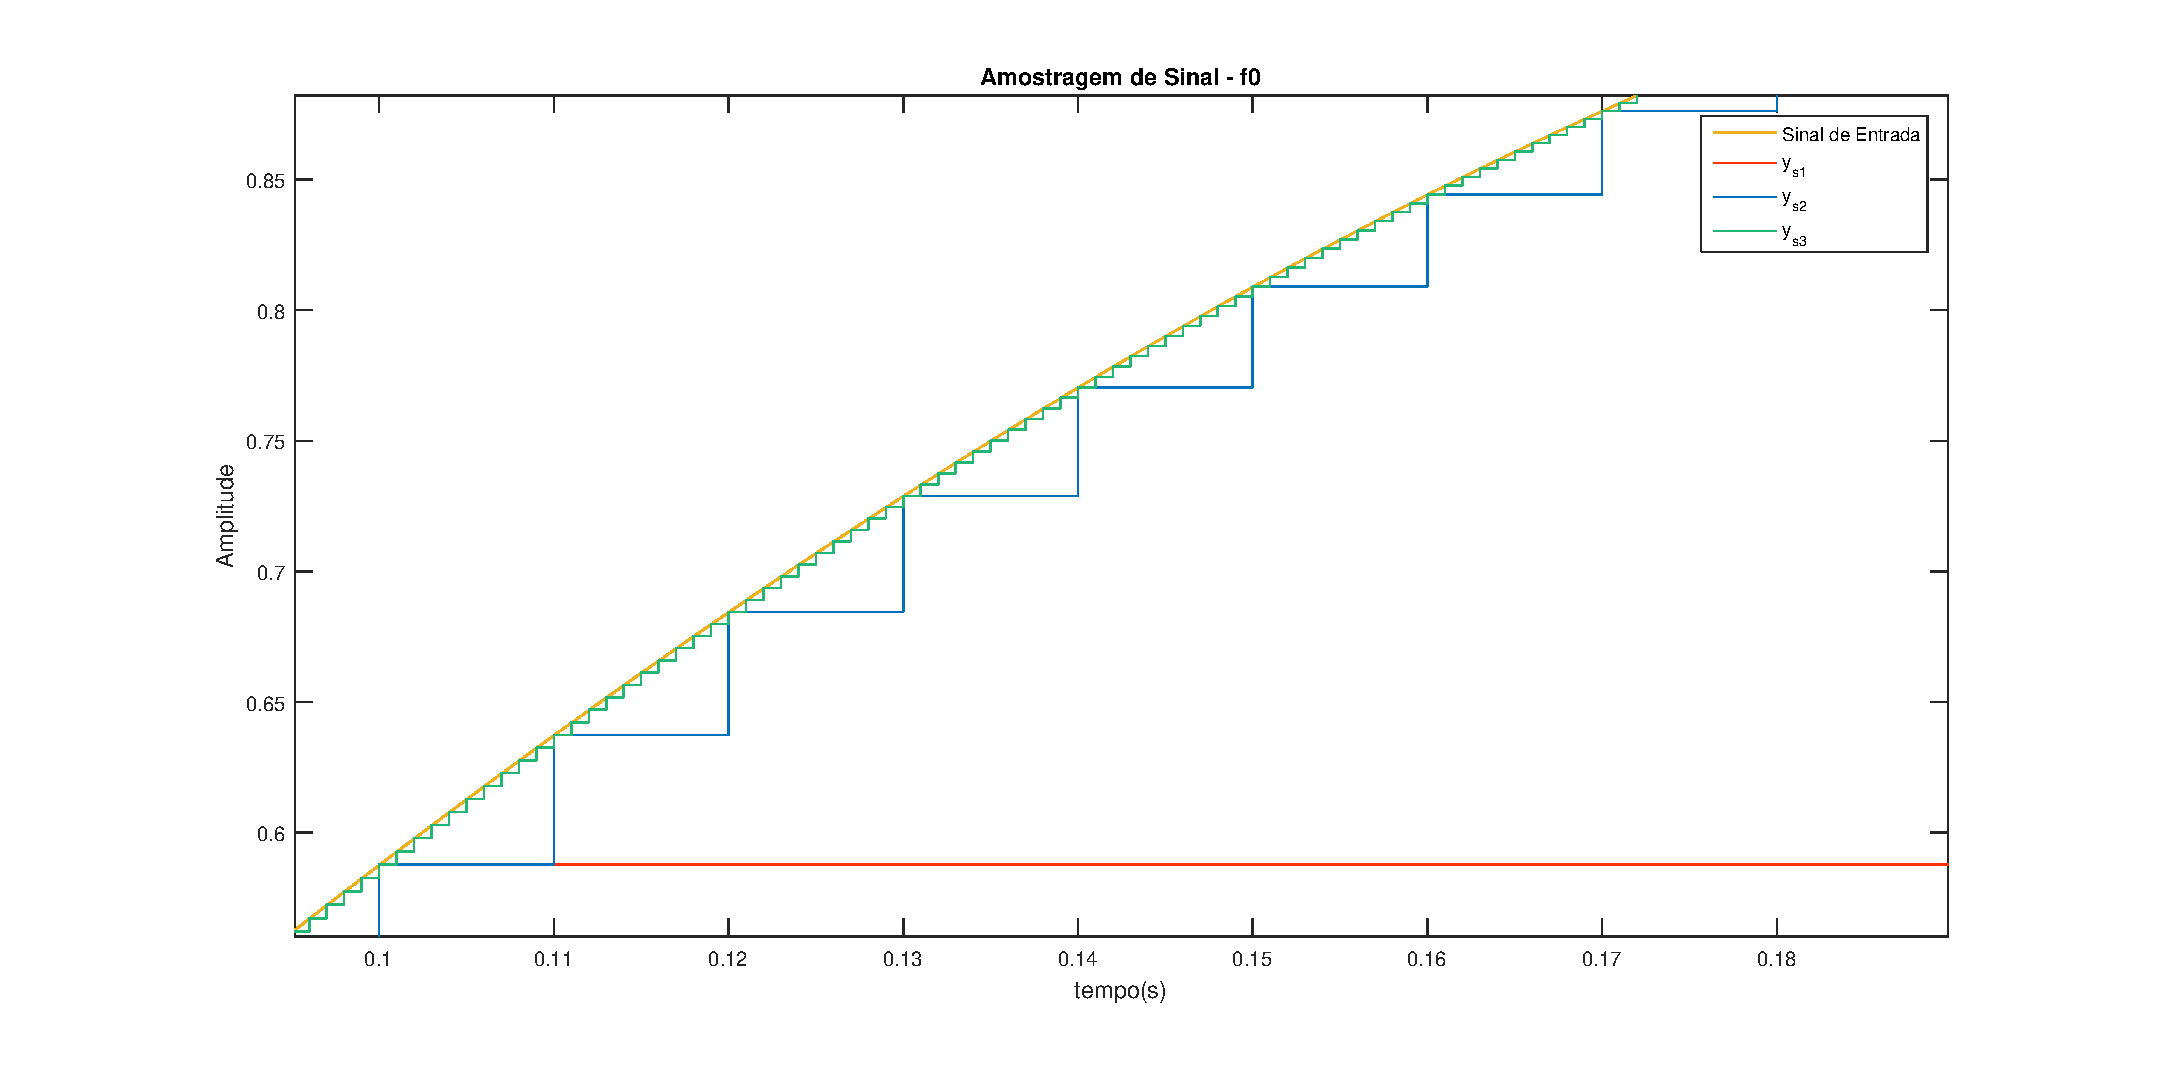
\includegraphics[scale = .45]{Imagens/pratica4_3.eps}
	\caption{Diagrama de blocos da prática 4.}
	\label{fig:pr4_esquema}
	\end{figure}
	
	\begin{figure}[!th]
		\centering
		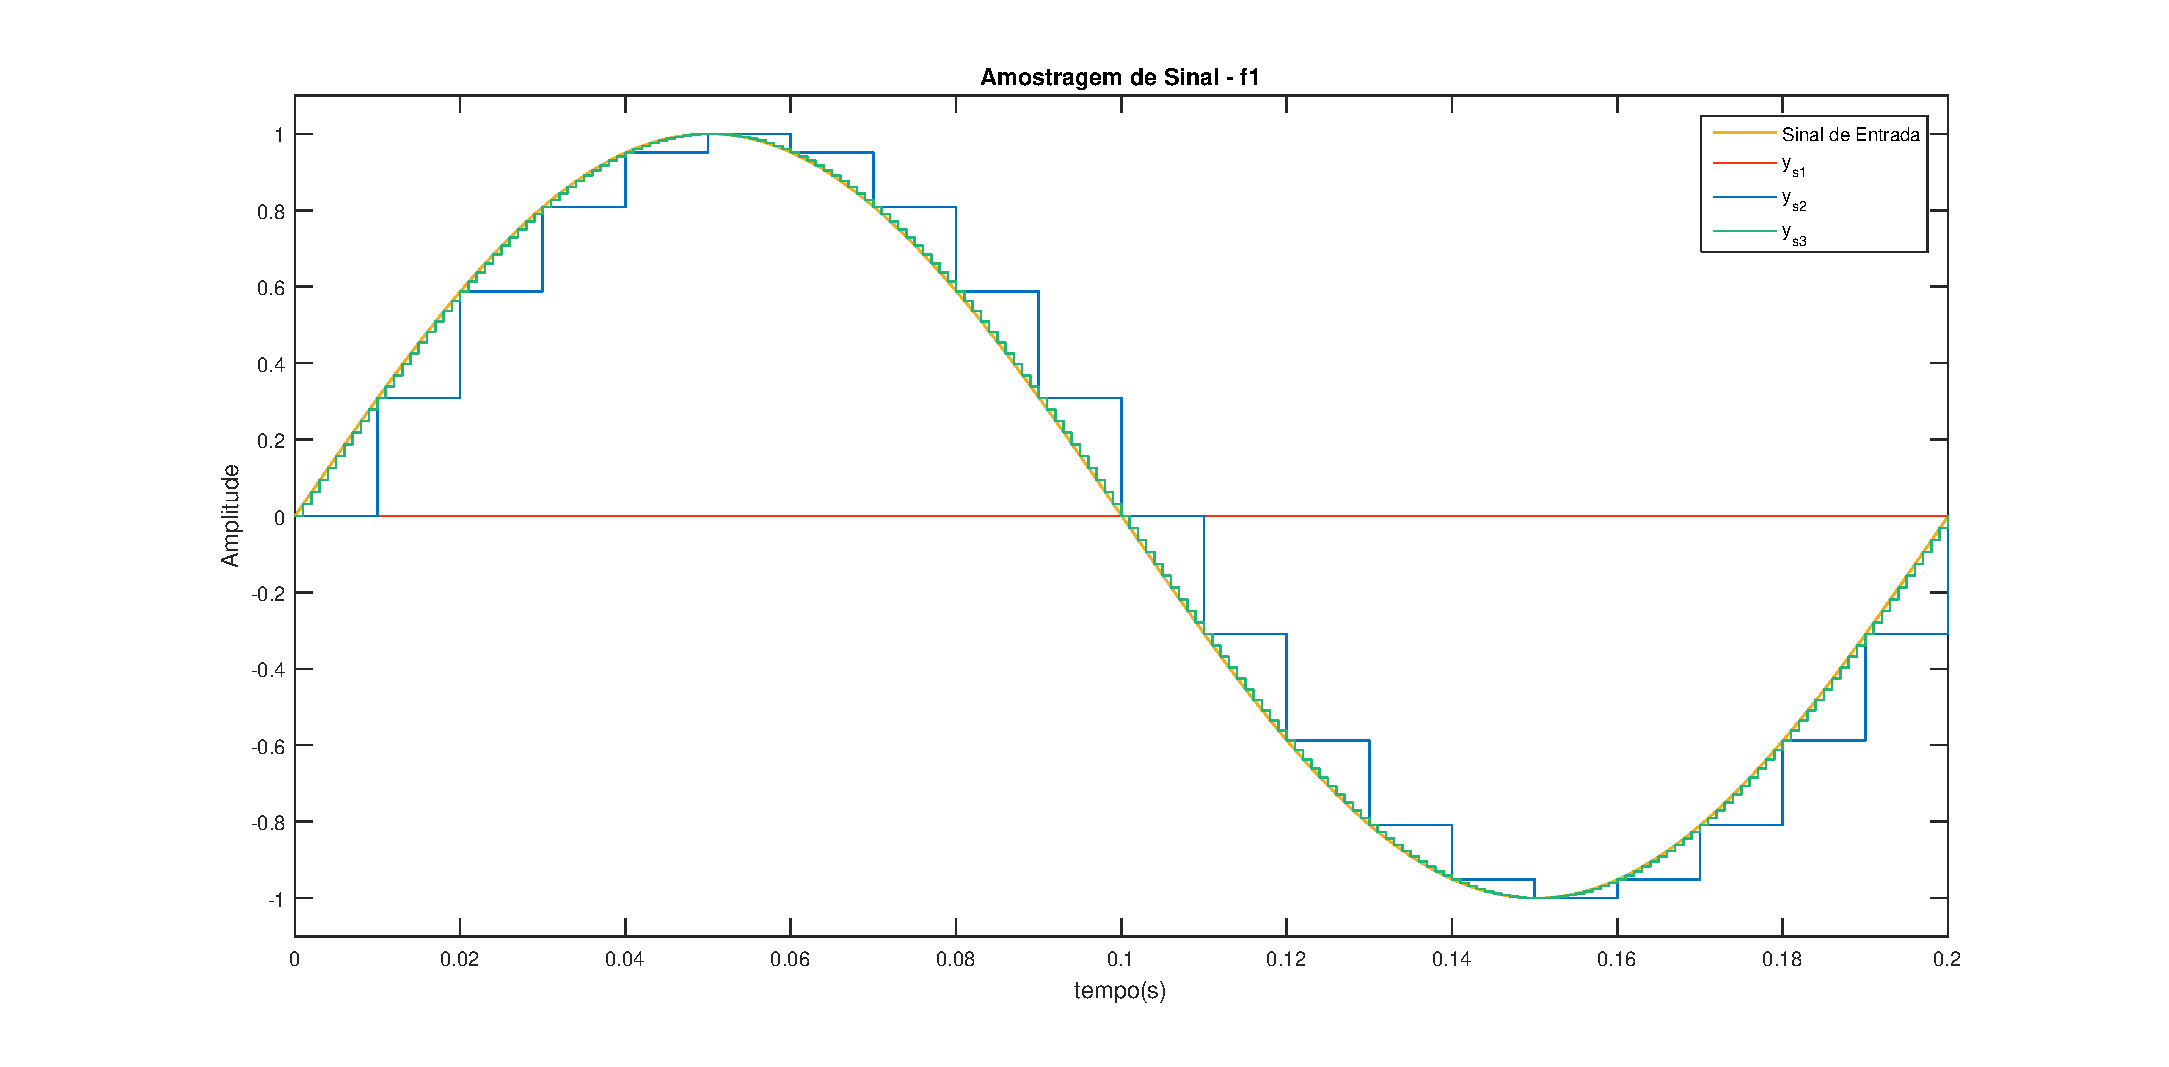
\includegraphics[scale = .45]{Imagens/pratica4_4.eps}
		\caption{Diagrama de blocos da prática 4.}
		\label{fig:pr4_esquema}
		\end{figure}
		
\begin{figure}[!th]
	\centering
	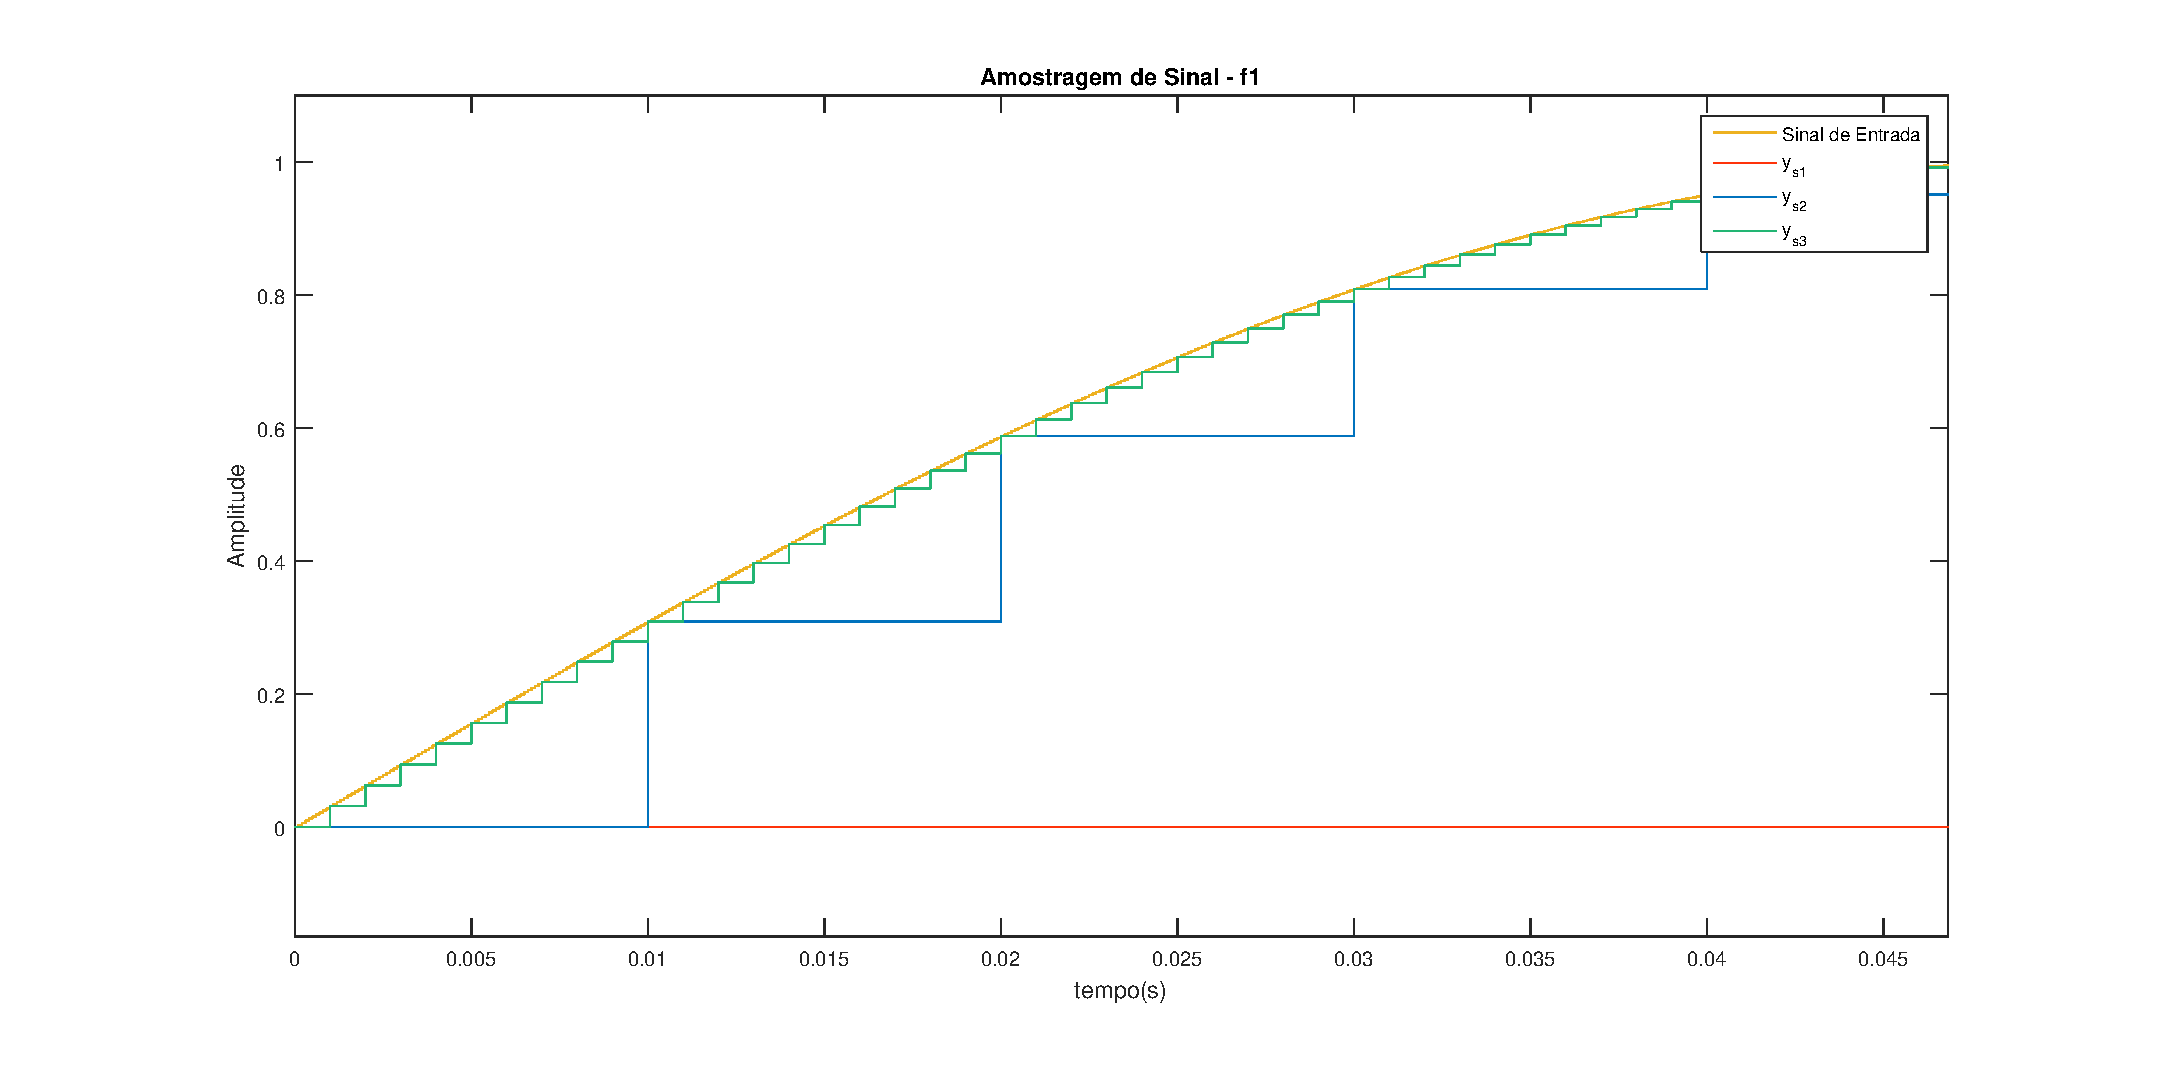
\includegraphics[scale = .45]{Imagens/pratica4_5.eps}
	\caption{Diagrama de blocos da prática 4.}
	\label{fig:pr4_esquema}
	\end{figure}
	
	\begin{figure}[!th]
		\centering
		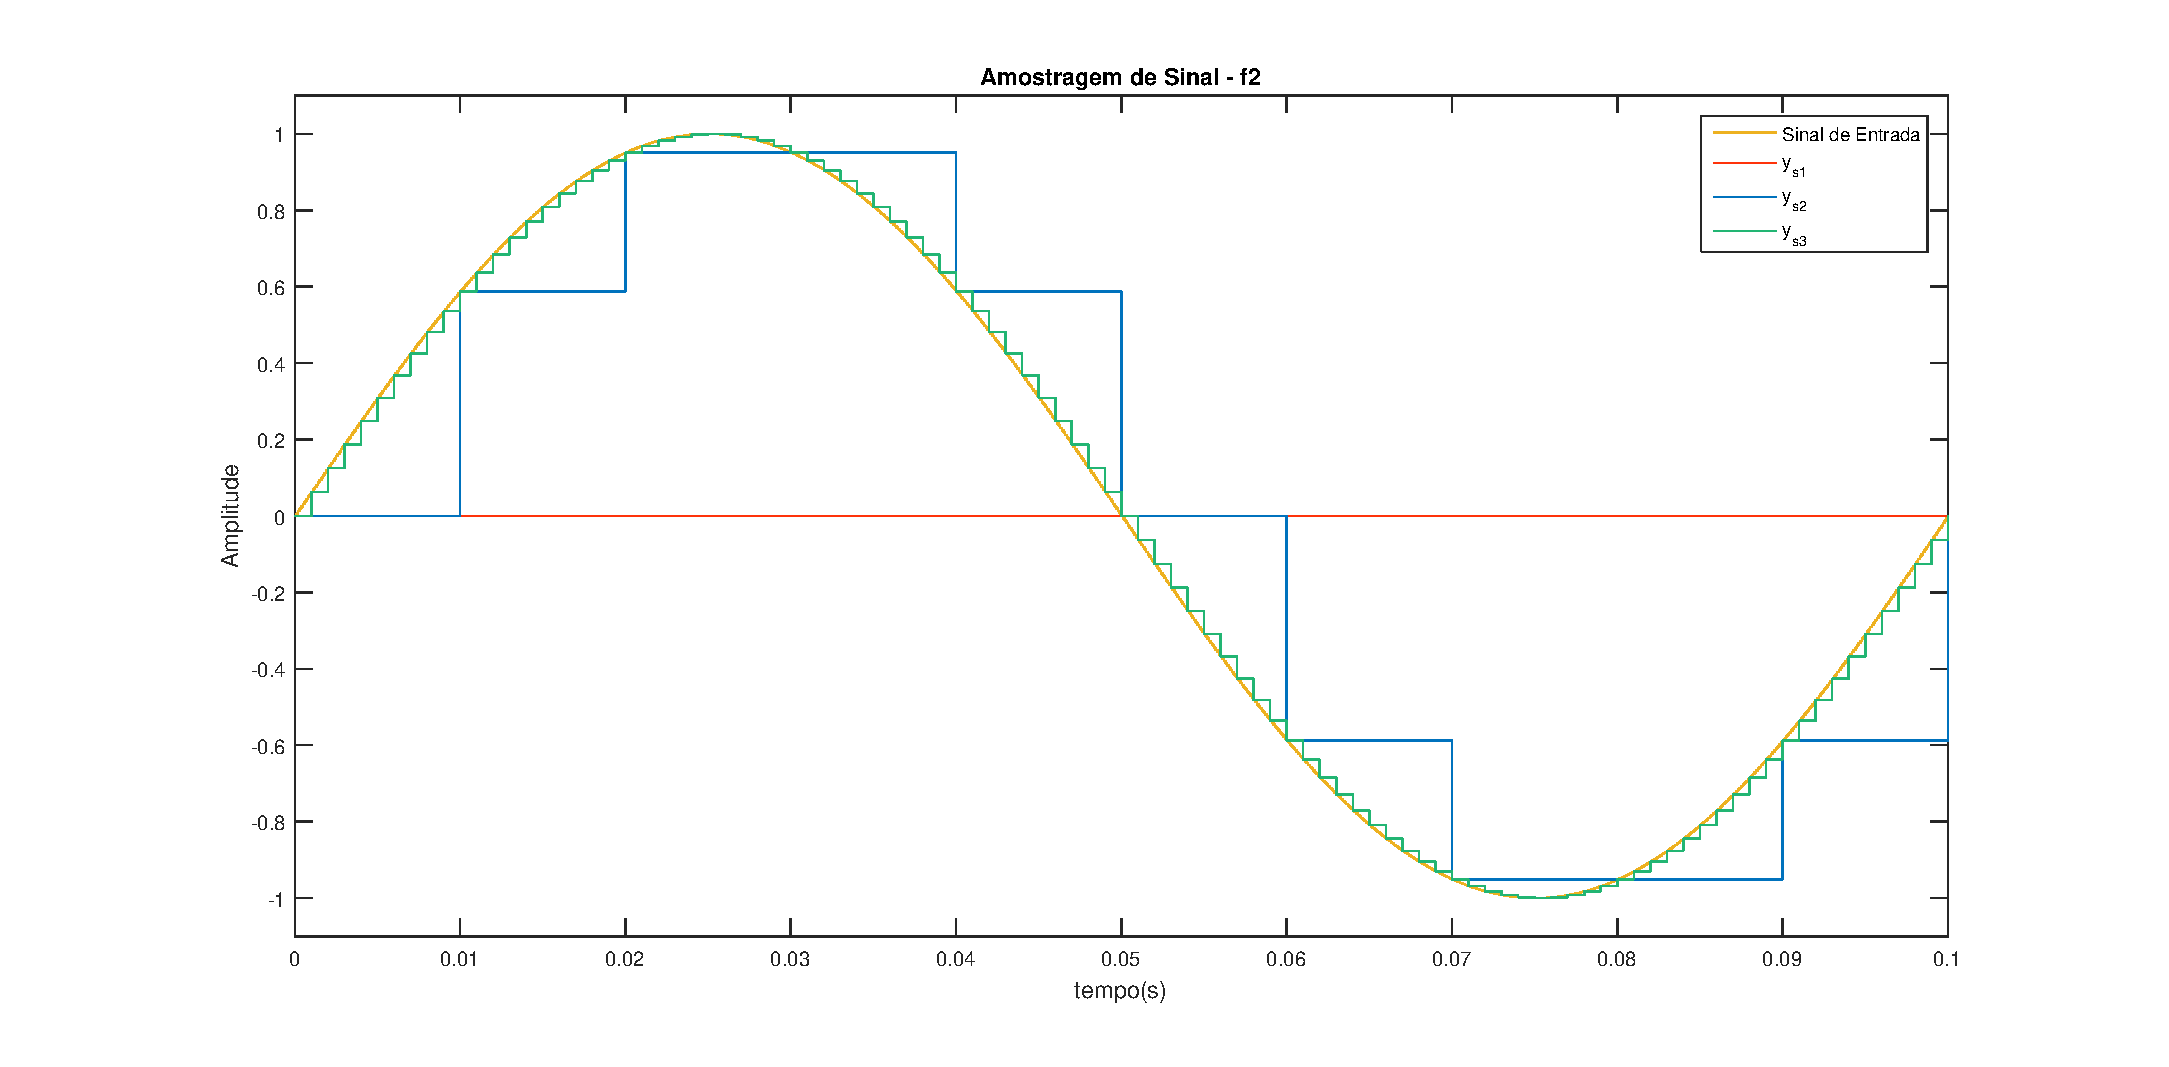
\includegraphics[scale = .45]{Imagens/pratica4_6.eps}
		\caption{Diagrama de blocos da prática 4.}
		\label{fig:pr4_esquema}
		\end{figure}